\documentclass[a4paper,10pt]{article}
\usepackage[margin=15mm]{geometry}
\usepackage{pgf,tikz}
\usepackage{subfig}
\usepackage{amsmath}
\usepackage{color}
\usepackage{amssymb}
\usepackage{noweb}
\usepackage{listings}
\usetikzlibrary{circuits.logic.US}
\usetikzlibrary{positioning}
\usetikzlibrary{matrix}
 
\definecolor{dkgreen}{rgb}{0,0.6,0}
\definecolor{gray}{rgb}{0.5,0.5,0.5}
\definecolor{mauve}{rgb}{0.58,0,0.82}

\lstset{ %
  language=Verilog,                % the language of the code
  basicstyle=\footnotesize,           % the size of the fonts that are used for the code
  numbers=left,                   % where to put the line-numbers
  numberstyle=\tiny\color{gray},  % the style that is used for the line-numbers
  stepnumber=2,                   % the step between two line-numbers. If it's 1, each line 
                                  % will be numbered
  numbersep=5pt,                  % how far the line-numbers are from the code
  backgroundcolor=\color{white},      % choose the background color. You must add \usepackage{color}
  showspaces=false,               % show spaces adding particular underscores
  showstringspaces=false,         % underline spaces within strings
  showtabs=false,                 % show tabs within strings adding particular underscores
%  frame=single,                   % adds a frame around the code
  rulecolor=\color{black},        % if not set, the frame-color may be changed on line-breaks within not-black text (e.g. commens (green here))
  tabsize=2,                      % sets default tabsize to 2 spaces
  captionpos=b,                   % sets the caption-position to bottom
  breaklines=true,                % sets automatic line breaking
  breakatwhitespace=false,        % sets if automatic breaks should only happen at whitespace
  title=\lstname,                   % show the filename of files included with \lstinputlisting;
                                  % also try caption instead of title
  keywordstyle=\color{blue},          % keyword style
  commentstyle=\color{dkgreen},       % comment style
  stringstyle=\color{mauve},         % string literal style
  escapeinside={\%*}{*)},            % if you want to add LaTeX within your code
  morekeywords={*,...}               % if you want to add more keywords to the set
}
\usepackage{amsthm}
\usepackage{hyperref}
\setlength{\parskip}{3mm}
\newtheorem{axiom}{Axiom}
\newtheorem{definition}{Definition}
\newtheorem{comment}{Comment}
\newtheorem{example}{Example}
\newtheorem{lemma}{Lemma}
\newtheorem{prop}{Property}
\newtheorem{problem}{Problem}
\newtheorem{remark}{Remark}
\newtheorem{theorem}{Theorem}

% Title Page
\title{Introduction to VHDL}
\author{Dilawar Singh}
\date{\today}

\begin{document}
\maketitle

\begin{abstract}
  
  This is not a tutorial of VHDL language. A minimal familiarity with grammar of
  computer languages are assumeed. It has been assumed that you have read the
  document posted on moodle about \textbf{proto-rtl} language.

\end{abstract}

\section{Introduction}
  
  Consider the following piece of hardware.
 
  \begin{figure}[h]
    %% Dilawar Singh (c) 2012 - 2013
%% Circuit macros to produce amazing quality circuits
%% More amazing than powerpuff girls.
\def\mux { -- ++(0,-1) node [above right] {$1$} -- ++(0.6,0.2) -- 
++(0,0.6) -- ++(-0.6,0.2) -- cycle};
\def\muxr { -- node [below left] {$1$} ++(1,0) -- ++(-0.2,-0.6) -- 
++(-0.6,0) -- ++(-0.2,0.6)  -- cycle}

%% Multiplexor 
%% 3 params : location, size, name.  
%% Note : To connect wires
%% to north, east, south and west one should also use .center with name.

\newcommand{\multiplexer}[3]{
\draw #1 -- ++(0,-#2/4)  node (#3_input1) at ++(0,0) {\scriptsize{\hspace{8pt}1}}
-- ++(0,-#2/2) node (#3_input2) at ++(0,0){\scriptsize{\hspace{8pt}0}} 
-- ++(0,-#2/4) -- ++(#2/2,#2/4)
-- ++(0,#2/4) node(#3_output) [] {}  -- ++(0,#2/4) 
-- ++(-#2/4,#2/8) node(#3_select) {} -- ++(-#2/4,#2/8)
}

%% Register 
%% 4 parama : location, width, height, name 
%% Note : To connect wires to north, east, south and west one should 
%% also use .center with name.
\newcommand{\register}[4]{
\draw #1 -- ++(#2/2,0) node(#4_north){} --++(#2/2,0) 
% eastern side
-- ++(0,-#3/2) node(#4_east){} -- ++(0,-#3/2) 
% southern side 
-- ++(-#2/2,0) node(#4_south){} --++(-#2/2,0) 
% label 
-- ++(0,#3) node at ($#1+(#2/2+0.1,-#3/2)$) {#4} 
% the western triangle
-- ++(0.6*#3, -0.5*#3) -- ++(-0.6*#3, -0.5*#3)
% the western anchor
-- ++(0,#3/2) node (#4_west) {}
}

%% Bus
%% 3 params : from, to, size 
\newcommand*{\bus}[4] {
\draw[->] #1 -- #2 node[midway]{\tiny{/}} 
    node [#3] {\scriptsize{#4}}
}

%% D flip-flop
%% 4 params : left bottom, width, height, label
\newcommand{\dflipflop}[4] {
\draw #1 -- ++(#2/2,0) node(#4_set) at ++(0,0) [above] {\scriptsize{S}}
-- ++(#2/2,0) 
% qbar 
-- ++(0,#3/3) node (#4_qbar) at ++(0,0) [left] {\scriptsize{$\bar{Q}$}}
-- ++(0,#3*2/3)
% q
-- ++(0,#3/3) node (#4_q) at ++(0,0) [left] {\scriptsize{${Q}$}}
-- ++(0,#3/3)
% reset 
-- ++(-#2/2,0) node (#4_reset) at ++(0,0) [below] {\scriptsize{R}}
-- ++(-#2/2,0)
% D
-- ++(0,-#3/3) node (#4_d) at ++(0,0) [right] {\scriptsize{D}}
-- ++(0,-#3*2/3)
%% clock
-- ++(0, -0.2) -- ++(0.2,0.2) -- ++(-0.2, 0.2) -- ++(0, -0.2) 
node (#4_clock) at ++(0,0) [right]  {}
%% clock enable
-- ++(0,-#3/3) node (#4_ce) at ++(0,0) [right] {\scriptsize{CE}}
-- cycle
}

    \begin{center}
      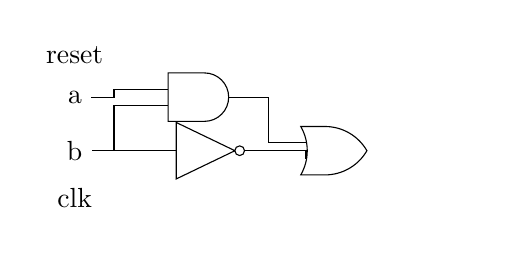
\begin{tikzpicture}[circuit logic US]
        %\dflipflop{(c.center)}{2}{2}{``DFF''};
        %% Draw the combinational logic.
        \matrix[column sep=7mm]
        {
          \node (reset) {reset}; & & & & \\
          \node (a) {a}; & \node[and gate] (a1) {}; &  & & \\ 
          \node (b) {b};  & \node[not gate] (n1) {};& \node[or gate] (o1) {}; & & \\
          \node (clk) {clk};  &  & & \\
        };
        % \dflipflop{(clk)}{1}{1}{dff};
        % \draw (reset) -| (dff_reset);
        \draw (a) -- ++(right:5mm) |- (a1.input 1);
        \draw (b) -- ++(right:5mm) |- (a1.input 2);
        \draw (b) -- ++(right:5mm) |- (n1.input);
        \draw (n1.output) -| (o1.input 2);
        \draw (a1.output) -- ++(right:5mm) |- (o1.input 1);
      \end{tikzpicture}
    \end{center}
    \caption{A small toy circuit. Describe it in proto-RTL.}
    \label{fig:circuit}
  \end{figure}

\end{document}          
